\documentclass[a4paper,openany]{book}

\usepackage{indentfirst}
\setlength{\parindent}{0em}
\usepackage{autobreak}
\allowdisplaybreaks
\usepackage{parskip}
\usepackage{geometry}
\geometry{top=3cm,bottom=3cm,left=2cm,right=2cm}
\usepackage{anyfontsize}
\usepackage{titlesec}
\titleformat{\chapter}{\bfseries}{\thechapter}{0em}{\LARGE}
\titlespacing*{\chapter}{0em}{-4em}{2em}
\usepackage{autobreak}
\allowdisplaybreaks
\linespread{1.25}
\raggedbottom

\usepackage{amsmath}
\usepackage[libertinus]{newtx}
\usepackage{bm}
\usepackage[cal=cm]{mathalpha}
\usepackage[mathb]{mathabx}

\usepackage{tikz}
\usetikzlibrary{arrows.meta,bending}
\usepackage{pgfplots}
\pgfplotsset{compat=newest}

\usepackage[fontset=none]{ctex}
\setCJKmainfont{Adobe Song Std}[BoldFont=Noto Sans CJK SC Medium, ItalicFont=Adobe Kaiti Std]
\newCJKfontfamily\kaishu{Adobe Kaiti Std}

\begin{document}

\title{\Huge\textbf{理论力学讲义}}
\author{\kaishu\Large 北京大学\ \ \ \ 张植竣}
\date{\kaishu\Large 2022年1月26日}
\maketitle

\chapter*{理论力学导论}

首先要介绍的是用\textbf{广义坐标}$q$和\textbf{广义速度}$\dot{q}$描述一个力学系统。广义坐标不一定具有长度的量纲，也可以是角度等其它物理量（这一点在Hamilton力学中体现更加明显），而广义速度是广义坐标对时间的导数。广义坐标的选取具有一定的任意性，如讨论弹簧振子时一般采用质点相对于平衡位置的位移作为广义坐标，而讨论圆周运动时则采用$(r,\theta)$作为两个广义坐标。

下一个概念是力学体系的\textbf{约束}。对于一个粒子数为$N$的三维力学体系，其总\textbf{自由度}数目（位移矢量$x_i$的总分量数）为$3N$。而如果对于一个力学系统，有以下$k$个方程：
\[
    f_m(x,t) = f_m(x_1,x_2,...,x_N,t) = 0,\quad m=1,2,...,k
\]
这样的方程称为\textbf{完整约束}，其余形式的约束（例如含有广义速度$\dot{q}$或者形式为不等式）统称为\textbf{非完整约束}。对于一个有$k$个完整约束的力学体系，其自由度个数为$M = 3N-k$。广义坐标是一个完整约束力学系统所有独立的自由度的一个最小集合。此时可以用：
\[
    x_i = x_i(q_1,q_2,...q_{3N-k},t),\quad i=1,2,...,N
\]
将位移矢量转化为广义坐标和时间的函数，于是可以用$3N-k$个广义坐标及其对应的广义速度和时间描述一个力学体系。\textbf{只有对于完整约束的力学体系，系统的自由度数目才等于广义坐标的数目}，非完整约束的体系中广义坐标的数目一般大于系统的自由度的数目。

于是可以引入所谓的\textbf{Lagrange量}$\boxed{\mathcal{L}(q,\dot{q},t)}$，对于一个保守体系（即能量守恒，时间反演后也对称），体系的Lagrange量可以取为：
\[
    \boxed{\mathcal{L}=T-V}
\]
此处$T$为体系的动能，$V$为体系的势能。以下考虑的力学问题中均不考虑摩擦力，故都是保守体系。

Lagrange量对时间的积分被称为一个体系的\textbf{作用量}$\boxed{S}$。如果一个力学体系在给定的时刻$t_1$和$t_2$分别由给定的广义坐标$q^{(1)}$和$q^{(2)}$描写，那么该力学体系的作用量$S$可以表达为联结这两个位形之间的各种可能轨道的\textbf{泛函}（自变量为函数的函数）：
\[
    \boxed{S = \int_{t_1}^{t_2} \mathcal{L}(q,\dot{q},t)\,\mathrm{d}t}
\]
对于任何一个力学体系都可以写出它的一个作用量，这是一个Lorentz标量（即在Lorentz变换下不变）。

理论力学的基本原理是\textbf{最小作用量原理}：
\[
    \delta S \equiv \int_{t_1}^{t_2} \mathcal{L}(q_c + \delta q,\dot{q}_c + \delta \dot{q},t)\,\mathrm{d}t - \int_{t_1}^{t_2} \mathcal{L}(q_c,\dot{q}_c,t)\,\mathrm{d}t = 0
\]
这里的$\delta$称为函数的\textbf{变分}，$q_c$是力学体系的真实运动轨道。

对于一元函数$y(x)$，$\delta y(x)$是一个这样的函数，其定义域与$y(x)$相同，并在定义域内满足$|\delta y(x)|<\varepsilon$，$|(\delta y)'(x)|<\varepsilon$，$\varepsilon$是一个任意小的数。

其运算法则如下：
\begin{align*}
    & \delta(\alpha F + \beta G) = \alpha \delta F + \beta \delta G,\quad \alpha,\beta \in\mathbb{C} \\
    & \delta(FG) = (\delta F)G + F(\delta G) \\
    & \delta(y') = (\delta y)' \\
    & \delta \int_a^b F\,\mathrm{d}x = \int_a^b (\delta F)\,\mathrm{d}x \\
    & \delta F(y,y',x) = \frac{\partial F}{\partial y}\delta y + \frac{\partial F}{\partial y'}\delta y'
\end{align*}
规定所有的轨道满足相同的边界条件，即$\delta q(t_1) = \delta q(t_2) = 0$，则导出：（这里用到了\textbf{Einstein约定}——重复的指标隐含着求和，下同）
\begin{align*}
    \delta S
    &= \delta \int_{t_1}^{t_2} \mathcal{L}(q,\dot{q},t)\,\mathrm{d}t \\
    &= \int_{t_1}^{t_2} \delta \mathcal{L}(q,\dot{q},t)\,\mathrm{d}t \\
    &= \int_{t_1}^{t_2} \left(\frac{\partial \mathcal{L}}{\partial q_i}\delta q_i + \frac{\partial \mathcal{L}}{\partial \dot{q}_i}\delta \dot{q}_i\right)\,\mathrm{d}t \\
    &= \int_{t_1}^{t_2} \left\{\frac{\partial \mathcal{L}}{\partial q_i}\delta q_i + \left[\frac{\mathrm{d}}{\mathrm{d}t}\left(\frac{\partial \mathcal{L}}{\partial \dot{q}_i}\delta q_i\right) - \delta q_i \cdot \frac{\mathrm{d}}{\mathrm{d}t}\left(\frac{\partial \mathcal{L}}{\partial \dot{q}_i}\right) \right]\right\}\,\mathrm{d}t \\
    &= \frac{\partial \mathcal{L}}{\partial \dot{q}_i}\delta q_i\bigg|_{t_1}^{t_2} + \int_{t_1}^{t_2} \mathrm{d}t\left[\frac{\partial \mathcal{L}}{\partial q_i} - \frac{\mathrm{d}}{\mathrm{d}t}\left(\frac{\partial \mathcal{L}}{\partial \dot{q}_i}\right)\right]\delta q_i \\
    &= 0
\end{align*}
上式第一项等于0，而第二项必须对\textbf{任意的}$\delta q_i$都等于0，又因为每个$\delta q_i$相互独立，唯一的可能是上式方括号中的量对于每一个$i$恒等于0（这在数学上称为\textbf{变分学基本引理}）。这样就得到\textbf{Euler-Lagrange方程}：
\[
    \boxed{\frac{\partial \mathcal{L}}{\partial q_i} - \frac{\mathrm{d}}{\mathrm{d}t}\left(\frac{\partial \mathcal{L}}{\partial \dot{q}_i}\right) = 0,\quad i=1,2,...,M}
\]
其中$M$为自由度个数。这是作用量$S$取极值的\textbf{必要条件}，其地位相当于经典力学中的运动方程——Newton第二定律。最小作用量原理和变分法告诉我们，一旦给定了一个力学体系的Lagrange量（作用量），体系的运动就由Euler-Lagrange方程决定。

\chapter*{对称性与守恒律}

如果系统具有\textbf{空间平移不变性}，即在变换$\bm{x}_2 = \bm{x}_1 + \Delta\bm{x}$下，系统的Lagrange量不变。这就要求：
\[
    \sum_i \left(\frac{\partial \mathcal{L}}{\partial x_i}\right) = 0
\]
由Euler-Lagrange方程，可以得到：
\[
    \frac{\mathrm{d}}{\mathrm{d}t}\left(\sum_i\frac{\partial \mathcal{L}}{\partial \dot{x}_i}\right) = 0
\]
定义\textbf{广义动量}，又称\textbf{正则动量}：
\[
    \boxed{\bm{p} = \sum_i\frac{\partial \mathcal{L}}{\partial \dot{x}_i}}
\]
则有$\dfrac{\mathrm{d}\bm{p}}{\mathrm{d}t} = 0$，即\textbf{广义动量对时间守恒}。

一般地，如果Lagrange量中不显含某一个广义坐标$q_i$（称之为\textbf{循环坐标}），则与之共轭的广义动量$p_i = \dfrac{\partial \mathcal{L}}{\partial \dot{q}_i}$一定守恒。

因此，Euler-Lagrange方程也可以写为：
\[
    \frac{\partial \mathcal{L}}{\partial q_i} = \frac{\mathrm{d}p_i}{\mathrm{d}t}\quad i=1,2,...,M
\]
由于这个方程与通常的Newton第二定律$\bm{F}_i = \dfrac{\mathrm{d}p_i}{\mathrm{d}t}$的相似性，$\dfrac{\partial \mathcal{L}}{\partial q_i}$又被称为相应的\textbf{广义力}。

如果系统具有\textbf{时间平移不变性}，即Lagrange量不显含时间。这就要求：
\[
    \frac{\partial \mathcal{L}(q,\dot{q})}{\partial t} = \frac{\partial \mathcal{L}}{\partial q_i}\,\dot{q}_i + \frac{\partial \mathcal{L}}{\partial \dot{q}_i}\ddot{q}_i = 0
\]
另一方面，考虑$p_i\dot{q}_i$对时间的导数，这里$p_i = \dfrac{\partial \mathcal{L}}{\partial \dot{q}_i}$是与$q_i$共轭的广义动量：
\[
    \frac{\mathrm{d}(p_i\dot{q}_i)}{\mathrm{d}t} = \frac{\mathrm{d}p_i}{\mathrm{d}t}\dot{q}_i + \frac{\mathrm{d}\dot{q}_i}{\mathrm{d}t}p_i
\]
由Euler-Lagrange方程，可以得到：
\[
    \frac{\partial \mathcal{L}}{\partial q_i}\dot{q}_i + \frac{\partial \mathcal{L}}{\partial \dot{q}_i}\ddot{q}_i
= \frac{\mathrm{d}}{\mathrm{d}t}\left(\frac{\partial \mathcal{L}}{\partial \dot{q}_i}\right)\dot{q}_i + p_i\frac{\mathrm{d}\dot{q}_i}{\mathrm{d}t}
= \frac{\mathrm{d}p_i}{\mathrm{d}t}\dot{q}_i + \frac{\mathrm{d}\dot{q}_i}{\mathrm{d}t}p_i
\]
定义系统的\textbf{Hamilton量}：
\[
    \boxed{\mathcal{H}(p,q,t) = p_i \dot{q}_i - \mathcal{L}}
\]
则$\dfrac{\mathrm{d}\mathcal{H}}{\mathrm{d}t} = 0$，即\textbf{Hamilton量对时间守恒}。

对于时间平移不变的保守体系，Hamilton量在数值上等于系统的能量，即动能与势能之和，即$\boxed{\mathcal{H} = T + V}$。

由$\mathcal{H} = p_i \dot{q}_i - \mathcal{L}$得：
\begin{align*}
    \mathrm{d}\mathcal{H}
    &= \dot{q}_i\mathrm{d}p_i + p_i\mathrm{d}\dot{q}_i - \mathrm{d}\mathcal{L} \\
    &= \dot{q}_i\mathrm{d}p_i + p_i\mathrm{d}\dot{q}_i - \left(\frac{\partial \mathcal{L}}{\partial q_i}\mathrm{d}q_i + \frac{\partial \mathcal{L}}{\partial \dot{q}_i}\mathrm{d}\dot{q}_i + \frac{\partial \mathcal{L}}{\partial t}\mathrm{d}t\right) \\
    &= \dot{q}_i\mathrm{d}p_i + p_i\mathrm{d}\dot{q}_i - \left(\dot{p}_i\mathrm{d}q_i + p_i\mathrm{d}\dot{q}_i + \frac{\partial \mathcal{L}}{\partial t}\mathrm{d}t\right) \\
    &= \dot{q}_i\mathrm{d}p_i - \dot{p}_i\mathrm{d}q_i - \frac{\partial \mathcal{L}}{\partial t}\mathrm{d}t
\end{align*}
与$\mathcal{H}$的全微分：
\[
    \mathrm{d}\mathcal{H} = \frac{\partial \mathcal{H}}{\partial p_i}\mathrm{d}p_i + \frac{\partial \mathcal{H}}{\partial q_i}\mathrm{d}q_i + \frac{\partial \mathcal{H}}{\partial t}\mathrm{d}t
\]
对比即得\textbf{Hamilton正则方程}：
\[
    \boxed{\dot{q}_i = \frac{\partial \mathcal{H}}{\partial p_i},\quad \dot{p}_i = -\frac{\partial \mathcal{H}}{\partial q_i}}
\]
如果系统具有\textbf{转动不变性}，即在无穷小转动$\Delta\bm{\phi}$下，有改变：$\Delta\bm{x} = \Delta\bm{\phi} \times \bm{x}$，$\Delta\bm{\dot{x}} = \Delta\bm{\phi} \times \bm{\dot{x}}$，系统的Lagrange量不变要求：
\[
    \frac{\mathrm{d}}{\mathrm{d}t}\left(\sum_i \bm{x_i} \times \bm{p_i}\right) = 0
\]
定义\textbf{角动量}：
\[
    \boxed{\bm{L} = \sum_i \bm{x_i} \times \bm{p_i}}
\]
则$\dfrac{\mathrm{d}\bm{L}}{\mathrm{d}t} = 0$，即\textbf{角动量对时间守恒}。

\textbf{一个体系的角动量一般依赖于坐标原点的选取}，如果将坐标原点平移一个常矢量$\Delta\bm{x}$，即在变换$\bm{x}_2 = \bm{x}_1 + \Delta\bm{x}$下，体系的总角动量会变为$\bm{L}_2 = \bm{L}_1 + \Delta\bm{x} \times \bm{p}$。

如果系统具有\textbf{尺度变换不变性}，即对系统作变换：$\bm{x}_2 = \lambda \bm{x}_1$，$t_2 = \mu t_1$，这相当于用不同的尺子度量长度和时间，称为\textbf{尺度变换}，此时系统的运动方程不变。在尺度变换下，我们考虑一类特殊的函数——\textbf{齐次函数}。据定义，$k$次齐次函数应满足：
\[
    \boxed{f(\lambda x_1, \lambda x_2,...,\lambda x_M) = \lambda^k f(x_1,x_2,...,x_M)}
\]
且有\textbf{Euler定理}（上式两边对$\lambda$求导并令$\lambda=1$）：
\[
    \boxed{\sum_i^M x_i \cdot \frac{\partial f}{\partial x_i} = kf}
\]
显然，动能$T = \dfrac{1}{2}m\bm{\dot{x}}^2$是速度的二次齐次函数，在尺度变换$\bm{x}_2 = \lambda \bm{x}_1$，$t_2 = \mu t_1$下，它应该变为$\left(\dfrac{\lambda}{\mu}\right)^2 T$。如果势能是坐标的$k$次齐次函数，尺度变换后系统的Lagrange量应该变为：
\[
    \mathcal{L} = \left(\frac{\lambda}{\mu}\right)^2 T - \lambda^k V
\]
令$\left(\dfrac{\lambda}{\mu}\right)^2 = \lambda^k$，得$\mu = \lambda^{1-\tfrac{k}{2}}$。这使得Lagrange量在尺度变换后只乘上一常数因子。而Lagrange量乘上一个常数因子并不会改变系统的运动方程（Euler-Lagrange方程），因此变换以后的系统的运动方程仍然形式上与原先的系统相同。这意味着这个系统具有几何上类似的轨道，在这些轨道上运行的特征时间与轨道尺度之间的比例也是固定的。具体来说，我们有：
\[
    \left(\frac{t'}{t}\right)^2 = \left(\frac{l'}{l}\right)^{2-k}
\]
其中$t'$，$l'$和$t$，$l$分别是两个相似轨道上的特征时间和特征尺度。在太阳系行星的公转周期运动中,势能$V(\bm{r}) = -\dfrac{GMm}{\bm{r}}$恰好是坐标的齐次函数（$k=-1$）。因此上式说明行星公转周期$T$的平方之比等于轨道尺寸（半长轴$a$）的立方之比，这就是著名的\textbf{Kepler第三定律}：
\[
    \boxed{\left(\frac{T'}{T}\right)^2 = \left(\frac{a'}{a}\right)^3}
\]
另外一个重要的例子是所谓\textbf{Virial定理}。我们考虑一个多粒子的力学体系并且假定体系局限在有限的空间范围内运动（例如太阳系中行星的运动、容器中空气分子的运动等）。由于体系的动能是速度的二次齐次函数，我们有：
\[
    2T = \sum_i \dot{x}_i \cdot p_i = \frac{\mathrm{d}}{\mathrm{d}t}\left(\sum_i x_i \cdot p_i\right) - \sum_i x_i \cdot \dot{p}_i
\]
现在我们将上式中的两边在很长的时间间隔$\tau$中平均。右边的第一项是时间的全微商,因此时间平均化为上式圆括号中的量在两个时间点之间的差在除以时间间隔$\tau$。由于系统局限在有限的区域运动，因此这个平均在长时间极限下为零（积分值有限，而$\lim\limits_{\tau \to \infty}\dfrac{1}{\tau} = 0$）：
\[
    \lim_{\tau \to \infty}\frac{1}{\tau}\int_0^\tau \frac{\mathrm{d}}{\mathrm{d}t}\left(\sum_i x_i \cdot p_i\right) = 0
\]
由于动能与坐标$x_i$无关，代入$\dot{p}_i = -\dfrac{\partial \mathcal{H}}{\partial x_i} = -\dfrac{\partial V}{\partial x_i}$得：
\[
    2\langle T \rangle = \left\langle \sum_i x_i \cdot \frac{\partial V}{\partial x_i} \right\rangle
\]
其中我们用$\langle\cdot\rangle$来表示对力学量的长时间平均值。

如果势能$V$是坐标的$k$次齐次函数，由Euler定理得：
\[
    2\langle T \rangle = k\langle V \rangle
\]
也就是说，系统的动能的平均与势能的平均有着简单的比例关系。这个关系的两个重要特例是有心力场中的Kepler问题（$k=-1$）和谐振子（$k=2$）。对于Kepler问题,动能平均是势能平均（小于零）的绝对值的一半，从而总能量是势能平均的一半；对于谐振子，动能平均与势能平均相等。

\chapter*{非惯性系的力学}

在经典力学中，所有的物理都体现在体系的经典运动方程中。也就是说，即使系统的Lagrange量或作用量改变了，只要体系的经典运动方程仍然保持不变，经典的物理就没有改变（这一点在量子体系中并不一定正确）。这个事实意味着一个经典力学体系的Lagrange量本身的数值并没有什么绝对的意义，只是由它导出的经典运动方程，即Euler-Lagrange方程才有意义。例如，我们完全可以在Lagrange量上加上一个\textbf{给定函数对于时间的全微分}：
\[
    \mathcal{L}'(q,\dot{q},t) = \mathcal{L}(q,\dot{q},t) + \frac{\mathrm{d}F(q,t)}{\mathrm{d}t} = \mathcal{L}(q,\dot{q},t) + \dot{F}
\]
显然，对于$\mathcal{L}'$来说，其作用量比$\mathcal{L}$的作用量多出$F(q,t)$在终止和初始时刻的差。但是由于我们考虑的变分$\delta q(t)$在端点处为零，因此加入$\dot{F}$并不会改变最小作用量原理所确定的力学体系的运动方程。也就是说，$\mathcal{L}'$与$\mathcal{L}$所确定的运动方程是完全一样的，两者在经典力学范畴内是完全等价的。这个事实我们在后面还会多次用到。两者在经典力学范畴内是完全等价的。这个事实我们在后面还会多次用到。

我们首先讨论一个\textbf{平动的非惯性系}。在一个惯性参照系$K_1$中，一个粒子的Lagrange量可以写为：
\[
    \mathcal{L}_1 = \frac{1}{2}m\bm{v}_1^2 - V
\]
现在我们假定有另外一个参照系$K_2$（不一定是惯性系），它相对于惯性系$K_1$以速度$\Delta\bm{v}(t)$平动。于是有：
\[
    \bm{v}_1 = \bm{v}_2 + \Delta\bm{v}
\]
粒子的Lagrange量可以写为：
\begin{align*}
    \mathcal{L}_2
    &= \frac{1}{2}m\bm{v}_1^2 - V \\
    &= \frac{1}{2}m\bm{v}_2^2 + m\bm{v}_2\cdot\Delta\bm{v} + \frac{1}{2}m\Delta\bm{v}^2 - V \\
    &= \frac{1}{2}m\bm{v}_2^2 + m\frac{\mathrm{d}\bm{x}_2}{\mathrm{d}t}\cdot\Delta\bm{v} + \frac{1}{2}m\Delta\bm{v}^2 - V \\
    &= \frac{1}{2}m\bm{v}_2^2 + \frac{\mathrm{d}}{\mathrm{d}t}(m\bm{x}_2\cdot\Delta\bm{v}) - m\frac{\mathrm{d}\Delta\bm{v}}{\mathrm{d}t}\cdot\bm{x}_2 + \frac{1}{2}m\Delta\bm{v}^2 - V
\end{align*}
将第二项，即给定函数对于时间的全微分去掉，可以化简为：
\[
    \mathcal{L}_2 = \frac{1}{2}m\bm{v}_2^2 - m\frac{\mathrm{d}\Delta\bm{v}}{\mathrm{d}t}\cdot\bm{x}_2 - V
\]
这个Lagrange量给出的运动方程为：
\[
    \boxed{m\bm{\dot{v}}_2 = -\frac{\partial V}{\partial\bm{x}_2} - m\frac{\mathrm{d}\Delta\bm{v}}{\mathrm{d}t}}
\]
右边的第二项$\boxed{-m\dfrac{\mathrm{d}\Delta\bm{v}}{\mathrm{d}t}}$被称为\textbf{惯性力}。

现在我们假定有另外一个参照系$K_3$（不一定是惯性系），它的原点与惯性系$K_1$的原点重合，它相对于惯性系$K_1$以角速度$\bm{\omega}(t)$转动。于是我们有：
\[
    \bm{v}_1 = \bm{v}_3 + \bm{\omega}\times\bm{x}_3
\]
则粒子的Lagrange量为：
\[
    \mathcal{L}_3 = \frac{1}{2}m\bm{v}_3^2 + m\bm{v}_3\cdot(\bm{\omega}\times\bm{x}_3) + \frac{1}{2}m(\bm{\omega}\times\bm{x}_3)^2 - V
\]
粒子的广义动量为：
\[
    \bm{p}_3 = \frac{\partial L_3}{\partial\bm{v}_3} = m\bm{v}_3 + m(\bm{\omega}\times\bm{x}_3)
\]
粒子的能量为：
\[
    \boxed{E_3 = \bm{p}_3\cdot\bm{v}_3 - L_3 = \frac{1}{2}m\bm{v}_3^2 - \frac{1}{2}m(\bm{\omega}\times\bm{x}_3)^2 + V}
\]
其中第二项能量$\boxed{-\dfrac{1}{2}m(\bm{\omega}\times\bm{x}_3)^2}$被称为\textbf{离心势能}。

同理，我们可以写出任意参照系中的质点的Lagrange量：
\[
    \boxed{\mathcal{L} = \frac{1}{2}m\bm{v}^2 + m\bm{v}\cdot(\bm{\omega}\times\bm{x}) + \frac{1}{2}m(\bm{\omega}\times\bm{x})^2 - m\frac{\mathrm{d}\Delta\bm{v}}{\mathrm{d}t}\cdot\bm{x} - V}
\]
及其运动方程：
\[
    \boxed{m\frac{\mathrm{d}\bm{v}}{\mathrm{d}t} = -\frac{\partial V}{\partial\bm{x}} - m\frac{\mathrm{d}\Delta\bm{v}}{\mathrm{d}t} + m\bm{x}\times\bm{\dot{\omega}} + 2m\bm{v}\times\bm{\omega} + m\bm{\omega}\times(\bm{x}\times\bm{\omega})}
\]
与惯性系中的运动方程比较我们发现，这个运动方程中多出了四项惯性力。第一项$- m\dfrac{\mathrm{d}\Delta\bm{v}}{\mathrm{d}t}$是非匀速的平动造成的；第二项$m\bm{x}\times\bm{\dot{\omega}}$是非匀速的转动引起的惯性力；第三项$2m\bm{v}\times\bm{\omega}$是著名的Coriolis力；第四项$m\bm{\omega}\times(\bm{x}\times\bm{\omega})$是惯性离心力。

\chapter*{中心力场}

考虑两个质量分别为$m_1$和$m_2$的粒子，通过一个有心势相互作用的力学体系。所谓\textbf{有心势}是指\textbf{两者相互作用的势能仅仅是两个粒子之间距离的函数}，相应的保守力构成一个\textbf{中心力场}，又称有心力场。因此，体系的Lagrange量可以写为：
\[
    \mathcal{L} = \frac{1}{2}m_1\bm{\dot{r}}_1^2 + \frac{1}{2}m_2\bm{\dot{r}}_2^2 - V(\|\bm{r}_1 - \bm{r}_2\|)
\]
为了方便我们取一个特定的惯性系使得两个粒子组成体系的质心速度为零。这样的参照系被称为\textbf{质心系}，并且质心就位于坐标架的原点。同时，我们引入两者的相对坐标$\bm{r} = \bm{r}_1 - \bm{r}_2$，于是：
\[
    \bm{r}_1 = \frac{m}{m_1}\bm{r},\quad \bm{r}_2 = \frac{m}{m_2}\bm{r}
\]
其中：
\[
    \boxed{m = \dfrac{m_1 m_2}{m_1 + m_2}}
\]
称为\textbf{约化质量}，又称\textbf{折合质量}。因此，只要求出了$\bm{r}(t)$我们就可以分别求出两个粒子的运动轨道。令$r = \|\bm{r}\|$，利用$m$和$\bm{r}$可以将Lagrange量变为一个等效的单粒子运动的形式：
\[
    \mathcal{L} = \frac{1}{2}m\bm{\dot{r}}^2 - V(r)
\]
Lagrange量的转动不变性决定了在这样的\textbf{一个中心力场中粒子的角动量一定守恒}。因此，我们可以将粒子的角动量取为沿$z$轴的方向。这样一来，粒子的运动轨道将完全处在$Oxy$平面内。采用更为方便的极坐标$(r,\phi)$，角速度$\omega = \dot{\phi}$，粒子的Lagrange量可以写为：
\[
    \mathcal{L} = \frac{1}{2}m\left(\dot{r}^2 + r^2\omega^2\right) - V(r)
\]
这个Lagrange量不显含坐标$\phi$，因此与$\phi$共轭的广义动量守恒，它实际上就是粒子沿$z$方向的角动量守恒：
\[
    \bm{L} = \frac{\partial \mathcal{L}}{\partial \bm{\omega}} = mr^2 \bm{\omega} = \mathrm{const.}
\]
这就是著名的\textbf{Kepler第二定律}，行星与太阳之间的连线在单位时间内扫过的面积是常数：
\[
    \boxed{\frac{\mathrm{d}S}{\mathrm{d}t} = \frac{1}{2}r^2 \omega = \frac{L}{2m} = \mathrm{const.}}
\]
这个定律实际上不依赖于相互作用势$V(r)$的具体形式，只要是有心势（角动量守恒）就可以了。

Lagrange量的时间平移对称性导致的另外一个守恒量是粒子的能量：
\[
    E
    = \frac{1}{2}m\left(\dot{r}^2 + r^2\omega^2\right) + V(r)
    = \frac{1}{2}m\dot{r}^2 + \frac{L^2}{2mr^2} + V(r)
    = \frac{1}{2}m\dot{r}^2 + V_{\mathrm{eff}}(r)
\]
其中：
\[
    \boxed{V_{\mathrm{eff}}(r) = V(r) + \frac{L^2}{2mr^2}}
\]
称为粒子的\textbf{有效势能}。

于是我们得到：
\[
    \frac{\mathrm{d}r}{\mathrm{d}t} = \sqrt{\frac{2}{m}\left[E-V(r)\right] - \frac{L^2}{m^2 r^2}}
\]
另一方面，由角动量定义得：
\[
    \dfrac{\mathrm{d}\phi}{\mathrm{d}t} = \dfrac{L}{mr^2}
\]
如果将上面两个方程相除，消去时间的微分$\mathrm{d}t$，则有：
\[
    \frac{\mathrm{d}r}{\mathrm{d}\phi} = \frac{1}{L}\sqrt{2mr^4[E-V(r)] - L^2 r^2}
\]
再积分，原则上就可以得到粒子轨道的表达式：
\[
    r(\phi) = r_0 + \int_{\phi_1}^{\phi_2} \frac{1}{L}\sqrt{2mr^4[E-V(r)] - L^2 r^2}\,\mathrm{d}\phi
\]

\chapter*{Kepler问题}

如果有心势的大小反比于距离：
\[
    V(r) = \frac{k}{r},\quad k \in \mathbb{R} \backslash \{0\}
\]
这时的力学问题称为\textbf{Kepler问题}。这类力学体系出现在以万有引力相互作用的行星与太阳之间，也可以存在于有库仑相互作用的两个点电荷之间。

在这里我们只讨论吸引势，此时粒子的势能和有效势能分别为：
\[
    V(r) = -\frac{m\alpha}{r},\quad V_{\mathrm{eff}}(r) = -\frac{m\alpha}{r} + \frac{L^2}{2mr^2}
\]
其中$\alpha > 0$为一个正的常数，对于万有引力，$\alpha = GM$。这个有效势能的特点是在$r \to 0$时，它趋于正无穷；在$r \to \infty$时，它从负的值趋于零。在区间$(0,\infty)$中，有效势能有一个极小值点。

因此，粒子的径向运动可以分为三种情况：如果粒子的能量$E>0$，那么粒子可以跑向无穷远，也就是说粒子的运动并不是束缚在力心周围有限的空间内，这时粒子的轨道是双曲线的一支。如果粒子的能量$E<0$，那么粒子的径向距离一定局限在一个有限的区间：$[r_{\mathrm{min}}, r_{\mathrm{max}}]$之内，这时粒子的运动一定被束缚在力心周围的一个有限区域内，不可能逃逸到无穷远，我们下面可以证明粒子的轨道是一个闭合的椭圆。如果粒子能量$E=0$，这时粒子的运动仍然可以逃逸到无穷，但运动轨道是一条抛物线。

联立能量与角动量方程：
\[
    \left\{
    \begin{aligned}
        & E = \frac{1}{2}m\dot{r}^2 - \frac{m\alpha}{r} + \frac{L^2}{2mr^2} \\
        & L = mr^2\dot{\phi}
    \end{aligned}
\right.
\]
化简得：
\[
    \mathrm{d}\phi = \frac{\mathrm{d}r}{r^2\sqrt{\left(\dfrac{e}{l_0}\right)^2 - \left(\dfrac{1}{r} - \dfrac{1}{l_0}\right)^2}}
\]
其中参数$l_0$与$e$由下式给出：
\[
    l_0 = \frac{b^2}{a} = \frac{L^2}{m^2\alpha},\quad e = \frac{c}{a} = \sqrt{1+\frac{2EL^2}{m^3\alpha^2}}
\]
积分可以给出粒子的轨道方程：
\[
    \boxed{r = \frac{l_0}{1+e\cos\phi}}
\]
这是极坐标中标准的圆锥曲线的方程，极坐标的原点位于圆锥曲线的焦点，$l_0$为椭圆的半通径，$e$为离心率。这里选择积分常数使得$\phi=0$对应于距离原点最近的点，该点在天文学中被称为\textbf{近日点}，$\phi=\pi$的点被称为\textbf{远日点}。

平面解析几何的知识告诉我们，当$e>1$时，轨道为双曲线；当$e=1$时为抛物线；当$0<e<1$时，轨道为椭圆；当$e=0$时，轨道是正圆。

在吸引势中，$E<0$的椭圆形轨道的结果正是\textbf{Kepler第一定律}。椭圆的半长轴$a$和半短轴$b$的值分别为：
\[
    \boxed{a = \frac{l_0}{1-e^2} = \frac{m\alpha}{2|E|},\quad b = \frac{l_0}{\sqrt{1-e^2}} = \frac{L}{\sqrt{2m|E|}}}
\]
椭圆轨道的近日点距离$r_{\mathrm{peri}}$和远日点距离$r_{\mathrm{apo}}$分别为：
\[
    r_{\mathrm{peri}} = a(1-e) = \frac{l_0}{1+e},\quad
r_{\mathrm{apo}} = a(1+e) = \frac{l_0}{1-e}
\]
由能量守恒和角动量守恒：
\[
    \frac{1}{2}mv_{\mathrm{peri}}^2 - \frac{m\alpha}{a(1-e)} = \frac{1}{2}mv_{\mathrm{apo}}^2 - \frac{m\alpha}{a(1+e)}
\]
\[
    ma(1-e)v_{\mathrm{peri}} = ma(1+e)v_{\mathrm{apo}}
\]
解得近日点和远日点处的速度：
\[
    v_{\mathrm{peri}} = \sqrt{\frac{\alpha}{a}\cdot\frac{1+e}{1-e}},\quad v_{\mathrm{apo}} = \sqrt{\frac{\alpha}{a}\cdot\frac{1-e}{1+e}}
\]
椭圆轨道的周期可以用椭圆的面积除以面积速度（即$v_S = \dfrac{1}{2}r^2\omega$）来确定：
\[
    T = \frac{\pi ab}{v_S} = 2\pi a\sqrt{\frac{a}{\alpha}}
\]
这其实就是\textbf{Kepler第三定律}：
\[
    \boxed{\frac{a^3}{T^2} = \frac{\alpha}{4\pi^2}}
\]
最后，我们简单讨论一下Kepler问题的特殊性。Kepler问题中轨道的闭合性实际上意味着距离反比有心势具有更高的对称性。这种对称性并不是由于时空的基本对称性，而是由于势能的特殊形式造成的，因此被称为\textbf{动力学对称}。动力学对称性的存在直接的后果就是有多余的守恒量，例如所谓\textbf{Laplace-Runge-Lenz矢量}（LRL矢量）：
\[
    \bm{M} = \bm{p}\times\bm{L} - m^2\alpha\frac{\bm{r}}{r}
\]
LRL矢量与离心率有密切关系。定义\textbf{离心率矢量}$\bm{e} = \dfrac{\bm{M}}{m^2\alpha}$，其大小等于离心率$e$，方向沿从焦点到近日点的方向：
\[
    \bm{e} = \frac{1}{m^2\alpha}(\bm{p}\times\bm{L}) - \frac{\bm{r}}{r}
\]
由$\bm{r}\cdot(\bm{p}\times\bm{L}) = \bm{L}\cdot(\bm{r}\times\bm{p}) = L^2$，$(\bm{p}\times\bm{L})^2 = p^2 L^2$（注意$\bm{p}$与$\bm{L}$垂直），以及$E = \dfrac{p^2}{2m} - \dfrac{m\alpha}{r}$，可以证明其大小等于离心率$e$：
\begin{align*}
    \bm{e}^2
    &= \frac{1}{m^4 \alpha^2}(\bm{p}\times\bm{L})^2 + \frac{\bm{r}^2}{r^2} - \frac{2}{m^2 \alpha}\bm{r}\cdot(\bm{p}\times\bm{L}) \\
    &= \frac{1}{m^4 \alpha^2}p^2 L^2 + 1 - \frac{2}{m^2 \alpha}L^2 \\
    &= 1 + \left(\frac{p^2}{2m} - \frac{m\alpha}{r}\right)\frac{2L^2}{m^3 \alpha^2} \\
    &= 1 + \frac{2EL^2}{m^2\alpha^2} \\
    &= e^2
\end{align*}
Laplace-Runge-Lenz矢量为常矢量（不随时间改变），验证如下：
\[
    \frac{\mathrm{d}\bm{M}}{\mathrm{d}t}
= \frac{\mathrm{d}}{\mathrm{d}t}(\bm{p}\times\bm{L}) - m^2\alpha\frac{\mathrm{d}}{\mathrm{d}t}\left(\frac{\bm{r}}{r}\right)
= \bm{p}\times\frac{\mathrm{d}\bm{L}}{\mathrm{d}t} - \frac{\mathrm{d}\bm{p}}{\mathrm{d}t}\times\bm{L} - m^2\alpha\frac{r\dot{\bm{r}} - \dot{r}\bm{r}}{r^2}
\]
注意角动量守恒：$\dfrac{\mathrm{d}\bm{L}}{\mathrm{d}t}=0$，且$\dfrac{\mathrm{d}\bm{p}}{\mathrm{d}t}=\bm{F}=-\dfrac{\partial V}{\partial r}=-\dfrac{m\alpha\bm{r}}{r^3}$，则有：
\begin{align*}
    \frac{\mathrm{d}\bm{M}}{\mathrm{d}t}
    &= -\frac{m\alpha}{r^3}\bm{r}\times\bm{L} - m^2\alpha\frac{r\dot{\bm{r}} - \dot{r}\bm{r}}{r^2} \\
    &= -\frac{m\alpha}{r^3}\bm{r}\times(\bm{r}\times\bm{p}) - m^2\alpha\frac{r\dot{\bm{r}} - \dot{r}\bm{r}}{r^2} \\
    &= -\frac{m^2\alpha}{r^3}\bm{r}\times(\bm{r}\times\dot{\bm{r}}) - m^2\alpha\frac{r\dot{\bm{r}} - \dot{r}\bm{r}}{r^2} \\
    &= -\frac{m^2\alpha}{r^3}[(\bm{r}\cdot\dot{\bm{r}})\bm{r}-r^2\dot{\bm{r}}] - m^2\alpha\frac{r\dot{\bm{r}} - \dot{r}\bm{r}}{r^2}
\end{align*}
代入恒等式：$\bm{r}\cdot\dot{\bm{r}} = \dfrac{1}{2}\dfrac{\mathrm{d}}{\mathrm{d}t}(\bm{r}\cdot\bm{r}) = \dfrac{1}{2}\dfrac{\mathrm{d}}{\mathrm{d}t}r^2 = r\dot{r}$，可得：
\begin{align*}
    \frac{\mathrm{d}\bm{M}}{\mathrm{d}t}
    &= -\frac{m^2\alpha}{r^3}(r\dot{r}\bm{r}-r^2\dot{\bm{r}}) - m^2\alpha\frac{r\dot{\bm{r}} - \dot{r}\bm{r}}{r^2} \\
    &= \frac{m^2\alpha}{r^2}(r\dot{\bm{r}}-\dot{r}\bm{r}) - m^2\alpha\frac{r\dot{\bm{r}} - \dot{r}\bm{r}}{r^2} \\
    &= 0
\end{align*}
这便证明了LRL矢量为常矢量。这个矢量是常矢量，保证了轨道的闭合。

\chapter*{潮汐现象}

我们考虑两个球形的、靠万有引力束缚在一起的星体，例如地球与太阳，或者地球与月亮。首先取质心系，坐标原点为两星体的质心C。为了进一步简化讨论，我们假定两个星体的运动轨道是一个正圆（这一点对于地日系统、地月系统差不多都是成立的）。如果两个星体公转的角速度为$\omega$。现在我们取另外一个相对于质心系旋转的参照系，其旋转的角速度正好等于$\omega$。在这个非惯性参照系中，两个星体是相对静止的。此处公转的角速度：
\begin{equation}
\omega = \sqrt{\frac{G(m_1 + m_2)}{R^3}}
\end{equation}

其中$R$代表两个体中心的距离，$m_1$和$m_2$为两个星体的质量。

\begin{figure}[ht!]
    \centering
    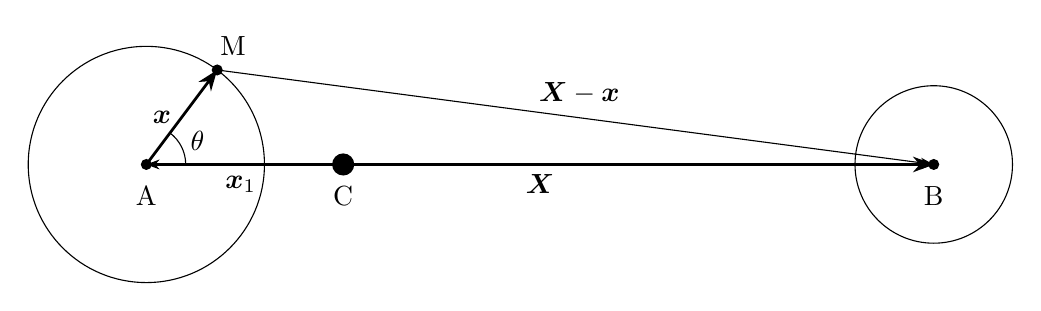
\begin{tikzpicture}[>=Stealth]
        \draw [->] (0,0) -- (-2.5,0);
        \draw [->] (0,0) -- (7.5,0);
        \draw [->,line width=1pt] (-2.5,0) -- (7.5,0);
        \fill (0,0) circle [radius=4pt];
        \fill (-2.5,0) circle [radius=2pt];
        \fill (7.5,0) circle [radius=2pt];
        \draw (0,-0.4) node {C};
        \draw (-2.5,-0.4) node {A};
        \draw (7.5,-0.4) node {B};
        \draw (-2.5,0) circle [radius=1.5cm];
        \draw (7.5,0) circle [radius=1cm];
        \draw [->,line width=1pt] (-2.5,0) -- (-1.6,1.2);
        \draw (-1.4,1.5) node {M};
        \draw [->] (-1.6,1.2) -- (7.5,0);
        \fill (-1.6,1.2) circle [radius=2pt];
        \draw (-1.3,-0.25) node {$\bm{x}_1$};
        \draw (2.5,-0.25) node {$\bm{X}$};
        \draw (-2.3,0.6) node {$\bm{x}$};
        \draw (3,0.9) node {$\bm{X}-\bm{x}$};
        \draw (-2,0) arc [start angle=0,radius=0.5,delta angle=53.130102];
        \draw (-1.85,0.3) node {$\theta$};
    \end{tikzpicture}
    \caption{\kaishu 潮汐问题的示意图（注意这里$\bm{X}=\protect\overrightarrow{AB}$，$\bm{x}_1=\protect\overrightarrow{CA}$）}
\end{figure}

潮汐问题主要需要处理图中星体A表面有液体的情形，液体会受两星体间的引力的影响而发生形状的变化。液体的表面（对于地球来讲就是海面）应该是一个等势面（达到稳态时动能为零）。我们将考察星体A表面任意一点处单位质量的能量。为此，设质心到星体A中心的矢量为$\bm{x}_1$，星体A的表面任意一点M相对于星体A的中心的位置矢量为$\bm{x}$，那么在两个星体以$\omega$角速度公转的非惯性系中，位于点$\bm{x}$处的单位质量$m$的势能可以写为：
\[
    V(\bm{x}) = -\frac{Gm_1 m}{\|\bm{x}\|} - \frac{Gm_2 m}{\|\bm{X} - \bm{x}\|} - \frac{1}{2}m\omega^2(\bm{x}_1+\bm{x})^2
\]
其中前两项分别是两个星体的万有引力造成的势能，$\bm{X} \equiv \bm{x}_2-\bm{x}_1$就是从星体A的中心指向星体B中心的位置矢量，第三项是非惯性系中的离心势能，其中$\bm{x}_1+\bm{x}$是从质心指向星体A表面任意一点M的位移矢量。记$r = \|\bm{x}\|$，$R = \|\bm{X}\|$。两个星体的位置矢量现在表达为：
\begin{equation}
    \bm{x}_1 = -\frac{m_2\bm{X}}{m_1+m_2},\quad \bm{x}_2 = \frac{m_1\bm{X}}{m_1+m_2}
\end{equation}
记$\bm{x}$与$\bm{X}$之间的夹角为$\theta$，则$\bm{x}$与$\bm{x}_1$之间的夹角为$\pi - \theta$，于是有：
\[
    \|\bm{X}-\bm{x}\| = \sqrt{\bm{X}_1^2 - 2\bm{X} \cdot \bm{x} + \bm{x}^2} = \sqrt{R^2 - 2rR\cos\theta + r^2}
\]
\[
    (\bm{x}_1 + \bm{x})^2 = \bm{x}_1^2 + 2\bm{x}_1 \cdot \bm{x} + \bm{x}^2 = \left(\frac{m_2 R}{m_1+m_2}\right)^2 - 2\left(\frac{m_2 R}{m_1+m_2}\right)r\cos\theta + r^2
\]
现在我们假定$R \gg r$，我们可以从Taylor展开：
\[
        (1+x)^a \approx 1 + ax + \frac{a(a-1)}{2}x^2
\]
及余弦定理：
\[
    \frac{1}{\|\bm{X}-\bm{x}\|} = \frac{1}{\sqrt{R^2 - 2rR\cos\theta + r^2}} = \frac{1}{R} \cdot \frac{1}{\sqrt{1-\dfrac{2r}{R}\cos\theta+\dfrac{r^2}{R^2}}}
\]
将$V(\bm{x})$的第二项展开：
\begin{equation}
    \frac{1}{\|\bm{X}-\bm{x}\|} \approx \frac{1}{R} + \frac{r}{R^2}\cos\theta - \frac{r^2}{2R^3} + \frac{3r^2}{2R^3}\cos^2\theta
\end{equation}
将(1)、(2)、(3)三式代入$V(\bm{x})$的表达式得：
\[
    \boxed{V(\bm{x}) = -\frac{Gm_1 m}{r} - \frac{Gm_2 m}{R} - \frac{1}{2}m\omega^2 r^2 - \frac{1}{2}m \omega^2\bm{x}_1^2 + \frac{Gm_2 m}{2R^3}r^2 - \frac{3Gm_2 m}{2R^3}r^2\cos^2\theta}
\]
上式中的前五项都不依赖于点$\bm{x}$在星体A表面的位置（$\theta$的值）。如果星体A表面是球体，这些项都是恒定的。但是，最后一项却依赖于点$\bm{x}$在球面的位置。具体来说，当$\bm{x}$位于两个星体的连线与星体A表面的交点时（也就是说矢量$\bm{x}$与矢量$\bm{X}$平行或反平行时），这一项的贡献会取最小值（势能$V(\bm{x})$最低），相反，当$\bm{x}$与连线方向$\bm{X}$垂直时，$V(\bm{x})$的最后一项取最大值（为零）。由于最后一项与前几项相比是小的，因此如果不考虑最后一项的贡献，势能在星体A表面的分布是均匀和各向同性的。如果考虑到最后一项的修正，那么势能在沿着两个星体中心连线的方向会比其他方向更低一些。因此，如果星体A表面具有流动性的液体物质，比如地球表面的海洋，那么这些流动性的液体就会比较倾向于集中到沿着两个星体中心连线的方向上去，这就造成了潮汐。$V(\bm{x})$的展开式还告诉我们，对地球上一个固定的地点来说，由于地球的自转，该地的引潮力一天之内大约会有两次（而不是一次！）相隔约半天时间的极大值（$\bm{x}$与$\bm{X}$平行或反平行，即$\theta=0^\circ$或$\theta=180^\circ$）。对于月球引起的潮汐，其相邻两次大潮的间隔是半个太阴日，即月球相邻两次上中天间隔的一半，约为$12^h 25^m$，略长于半个太阳日。

引起潮汐的力被称为\textbf{引潮力}。它来源于星体B对星体A引力的空间不均匀性：
\[
    F = \frac{\mathrm{d}}{\mathrm{d}R}\left(\frac{Gm_2 m}{R^2}\right) = -\frac{2Gm_2 m}{R^3}
\]
则有：
\[
    \boxed{\Delta F = \frac{2Gm_2 m}{R^3}\Delta r}
\]
公式告诉我们，引潮力$\Delta F$取决于星体B的质量$m_2$（与之成正比）以及它与星体A的距离$R$（与其三次方成反比）。具体的分析表明：太阳和月亮都会对地球上的潮汐造成影响，但是由于月亮比较近，因此月亮的影响反而更重要一些，尽管它的质量远小于太阳的质量。

对于星体A（在这里是卫星）上最靠近星体B（在这里是主星）的质点，由于$r \ll R$，有：
\[
    f = \frac{2Gm_2 m}{R^3}r
\]
这个力与星体A自身的引力抗衡（忽略轨道公转），当两个力平衡时，该质点恰好脱离星体A表面：
\[
    \frac{2Gm_2 m}{R^3}r = \frac{Gm_1 m}{r^2}
\]
此时星体A开始被潮汐力所撕碎，对应的星体间距离为：
\[
    \boxed{R_0 = r_A\sqrt[3]{\frac{2m_2}{m_1}} = 1.26r_A\sqrt[3]{\frac{m_2}{m_1}}}
\]
这里的$r_A = r$是星体A（卫星）的半径。另一种表示方法是用星体B（主星）的半径表示，这需要使用两个星体的密度：
\[
    \boxed{R_0 = r_B\sqrt[3]{\frac{2\rho_2}{\rho_1}} = 1.26r_B\sqrt[3]{\frac{\rho_2}{\rho_1}}}
\]
这个$R_0$被称为\textbf{Roche半径}。

\chapter*{受限三体问题与Lagrange点}

在经典牛顿力学的框架中，所谓\textbf{三体问题}是指任意质量的三个质点，假定相互之间只有牛顿万有引力的相互作用，该三体系统在任意初始条件下运动轨迹的求解问题。这个问题实际上远比两体问题复杂得多。事实上，对于一般的三体问题不可能有完整的解析解（1887年由数学家Heinrich Bruns和Henri Poincaré首先证明）。一般的经典三体问题无法解析求解不意味着在一些特殊的构型下可以求解。下面我们就来讨论一大类非常有实际应用背景的情形：三个物体A、B、C的质量分别记为$m_1$、$m_2$和$m$，其中两个物体的质量远大于第三个物体的质量:
\[
    m_1 \gg m,\quad m_2 \gg m
\]
在这种情形下，最轻的质量所产生的引力场对于另外两个大质量物体的运动之影响完全可以忽略。也就是说，这个问题其实可以化简为两个大质量物体$m_1$和$m_2$的两体问题，它们的轨道由前面讨论的Kepler问题的解给出；而最轻的质量$m$只是在$m_1$和$m_2$所形成的固定的引力场之中运动而已。这类问题的最典型的应用就是考虑地球、月球和人造卫星之间的三体问题，或者太阳、地球、卫星之间的三体问题。无论是哪一类，人造卫星的质量都比太阳、地球或月球要小很多，因此它的存在并不会对日地或者月地的正常轨道有任何可观测的影响。我们称这类问题为\textbf{受限三体问题}。

尽管对于$m_1$和$m_2$构成的两体系统来说，其任意的圆锥曲线的轨道都是可能的，为了与实际更接近些，我们还是加上两者实际上按照圆轨道运行。这个假设不仅仅对于月地系统是正确的，而且对于太阳系的各个行星与太阳构成的系统基本上也都是对的。从上节的讨论我们知道，选取一个与两个星体一同转动的非惯性系是方便的。这个转动系的原点可以选择在两个星体的质心位置，并设$Oxy$平面即为它们的轨道平面，则转动的角速度沿$\bm{\hat{z}}$方向：
\[
    \bm{\omega} = \sqrt{\frac{G(m_1 + m_2)}{R^3}}\bm{\hat{z}}
\]
除了忽略掉质量$m$对$m_1$和$m_2$的运动的影响之外，结合具体的情况我们还可以假设两个星体的质量也有比较大的差距。我们约定：
\[
    m_1 \gg m_2 \gg m
\]
注意，这个假设虽然原则上并不是必须的。但是由于实际的应用中往往都可以得到满足，因此它可以大大简化我们的计算过程。

因此，对于任何有实际应用的受限三体系统而言，我们都可以令
\[
    \varepsilon = \frac{m_2}{m_1} \ll 1
\]
这将极大地简化我们的计算。本节将对这类特殊的三体问题做一个简要的介绍。

选取两个星体的质心为坐标原点并假定两个星体的运动在$Oxy$平面内。现在我们转换到与两个星体一起均匀旋转的非惯性系之中。为了简化讨论，我们选择两个星体的连线为$x$轴，两个星体之间的距离为$R$，星体A（质量较大者）、星体B（质量较小者）的坐标分别为：
\[
    \bm{x}_1 = (r_1,0,0),\quad \bm{x}_2 = (-r_2,0,0)
\]
其中：
\[
    r_1 = \frac{m_2}{m_1+m_2}R,\quad r_2 = \frac{m_1}{m_1+m_2}R
\]
对于这个特殊的问题选取一个合适的单位制是方便的。我们首先选取长度单位，使得$R=1$。换句话说，所有的长度量都按照$R$来度量。我们同时还可以选择时间的度量单位，使得公转角速度$\omega = 2\pi$（对于太阳系，这相当于取AU和回归年为单位）。由于我们考虑受两个星体引力影响的另一个质量为$m$的质点的运动，我们可以方便地将该质点的质量取为质量单位，即$m = 1$。

记质点的坐标为$\bm{x} = (x,y,z)$。在旋转参照系中质点$m$的有效势能由引力势能和离心势能两部分构成：
\[
    V_{\mathrm{eff}}(\bm{x}) = V(x) - \frac{1}{2}\left(\bm{\omega}\times\bm{x}\right)^2
\]
将有效势能用坐标$(x,y,z)$具体写出来为：
\[
    V_{\mathrm{eff}}(x,y,z) = -\frac{1}{2}\omega^2(x^2 + y^2) - \frac{Gm_1}{\sqrt{(x-r_1)^2 + y^2 + z^2}} - \frac{Gm_2}{\sqrt{(x+r_2)^2 + y^2 + z^2}}
\]
默认三个天体都在$z=0$的轨道平面上运动，可以化简为：
\[
    V_{\mathrm{eff}}(x,y) = -\frac{1}{2}\omega^2(x^2 + y^2) - \frac{Gm_1}{\sqrt{(x-r_1)^2 + y^2}} - \frac{Gm_2}{\sqrt{(x+r_2)^2 + y^2}}
\]
有效势能的等势面是三维空间的闭合曲面，称为\textbf{Roche等势面族}。下图所示为Roche等势面族在轨道平面（$z=0$）的截面图。

\begin{figure}[ht!]
    \centering
    \begin{tikzpicture}
        \begin{axis}[
        view={0}{90},
        samples=1000,
        domain=-3:3,
        axis equal=true,
        axis lines=middle,
        xtick=\empty,ytick=\empty,
        max=3,min=-3,
        xlabel={$x$},ylabel={$y$},
        width=7cm, height=7cm,
        ]
        \addplot3 [contour lua={levels={1.4, 1.42, 1.5, 1.6456751, 1.7782065, 1.9600748, 2.5, 3.5}, labels=false, draw color=black}] {0.5*(x^2+y^2) + 0.7/(sqrt((x-0.3)^2+y^2)) + 0.3/(sqrt((x+0.7)^2+y^2))};
        \addplot3[only marks, mark size=3.5pt] coordinates {(0.3,0,0)};
        \addplot3[only marks, mark size=1.5pt] coordinates {(-0.7,0,0)};
        \addplot[only marks, mark size=0.8pt] coordinates {(-0.28613,0) (-1.25673,0) (1.12321,0) (-0.2,-0.8660254) (-0.2,0.8660254)};
        \end{axis}
    \end{tikzpicture}
    \caption{\kaishu Roche等势面族在轨道平面的截面图}
\end{figure}

%\begin{tikzpicture}[>=Stealth]
%    \draw [->] (-3.5,0) -- (3.5,0);
%    \draw [->] (0,-3) -- (0,3);
%    \draw (3.3,-0.25) node {$x$};
%    \draw (-0.25,2.8) node {$y$};
%    \foreach \V in {1.4, 1.42, 1.5, 1.6456751, 1.7782065, 1.9600748, 2.5, 3.5}
%    \draw plot[raw gnuplot] function{
%    f(x,y) = 0.5*(x**2+y**2) + 0.7/(sqrt((x-0.3)**2+y**2)) + 0.3/(sqrt((x+0.7)**2+y**2)) - \V;
%    set xrange [-4:4];
%    set yrange [-4:4];
%    set view 0,0;
%    set isosample 1000, 1000;
%    set sample 1000, 1000;
%    set size square;
%    set contour base;
%    set cntrparam levels incre 0,0.1,0;
%    unset surface;
%    splot f(x,y);
%    };
%    \fill (0.3,0) circle [radius=3.5pt];
%    \fill (-0.7,0) circle [radius=1.5pt];
%    \fill (-0.28613,0) circle [radius=1pt];
%    \fill (-1.25673,0) circle [radius=1pt];
%    \fill (1.12321,0) circle [radius=1pt];
%    \fill (-0.2,0.8660254) circle [radius=1pt];
%    \fill (-0.2,-0.8660254) circle [radius=1pt];
%\end{tikzpicture}

在等势面上的任意一点，质点$m$所受到的有效力$\bm{F}_{\mathrm{eff}}$（引力加惯性离心力）总是垂直于等势面。因此，当一个质点沿着等势面运动时，有效力不做功，也就是说质点可以沿等势面自由运动。

在有效势能的极值点处：
\[
    \bm{F}_{\mathrm{eff}} = -\frac{\partial V_{\mathrm{eff}}(\bm{x})}{\partial\bm{x}} = 0
\]
因此，如果一个质点在某个时刻恰好静止于这些极值点处，它将永远停留在那里。因为在这些点处\textbf{惯性离心力和引力刚好平衡相消}。这些使得有效势能$V_{\mathrm{eff}}(\bm{x})$取极值的点被统称为\textbf{Lagrange点}。

下面我们寻找有效势能的极值点，即Lagrange点$\bm{x_L} = (x_L,y_L)$所满足的方程。

对有效势能求导数并令其为零得到：
\[
    \tag{$\ast$}
\left\{
\begin{aligned}
    &\omega^2 x_L = \frac{Gm_1(x_L-r_1)}{\left(\sqrt{(x-r_1)^2 + y^2}\right)^3} + \frac{Gm_2(x_L+r_2)}{\left(\sqrt{(x+r_2)^2 + y^2}\right)^3} \\
    &\omega^2 y_L = \frac{Gm_1y_L}{\left(\sqrt{(x-r_1)^2 + y^2}\right)^3} + \frac{Gm_2y_L}{\left(\sqrt{(x+r_2)^2 + y^2}\right)^3}
\end{aligned}
\right.
\]
我们看到Lagrange点大致可以分为两类：一类是位于两个星体连线（即$x$轴）上的，满足$y_L = 0$，另一类则是不在两星体连线上的，即$y_L \neq 0$。

首先看$y_L = 0$（共线）的Lagrange点。这时候极值方程的第二个方程自动得到满足。第一个方程在令$y_L = 0$后化简为：
\[
    x_L = \left(\frac{Gm_1}{\omega^2}\right)\frac{x_L-r_1}{|x_L-r_1|^3} + \left(\frac{Gm_2}{\omega^2}\right)\frac{x_L+r_2}{|x_L+r_2|^3}
\]
注意到：
\[
    r_1 = \frac{m_2}{m_1+m_2} = \frac{Gm_2}{\omega^2},\quad
r_2 = \frac{m_1}{m_1+m_2} = \frac{Gm_1}{\omega^2}
\]
则有：
\[
    x_L = f(x_L) = \frac{r_2(x_L-r_1)}{|x_L-r_1|^3} + \frac{r_1(x_L+r_2)}{|x_L+r_2|^3}
\]
这是一个关于$x_L$的五次方程，也就是说它不可能有根式解。按照通常的约定，$L_1$是位于两个星体之间的Lagrange点，$L_2$是在较小质量星体外侧的Lagrange点，$L_3$则是较大质量星体外侧的Lagrange点。据此规定正负号，三个Lagrange点满足的方程分别为：
\begin{align*}
    &L_1:\quad x_1 = -\frac{r_2}{(x_1-r_1)^2} + \frac{r_1}{(x_1+r_2)^2} \\
    &L_2:\quad x_2 = -\frac{r_2}{(x_2-r_1)^2} - \frac{r_1}{(x_2+r_2)^2} \\
    &L_3:\quad x_3 = \frac{r_2}{(x_3-r_1)^2} + \frac{r_1}{(x_3+r_2)^2}
\end{align*}
在零级近似下，$r_1=0$，$r_2=1$，此时显然解为：
\[
    x_1^{(0)} = x_2^{(0)} = -1,\quad x_3^{(0)} = 1
\]
这是完全符合预期的。因为如果忽略小星体的质量，则质心位置基本与大星体位置重合，这点我们取为原点。小星体位于绕大星体距离为1的圆轨道上。现在我们将$\varepsilon$很小但不等于零时的完整解表达为：
\[
    x_L = x_L^{(0)} + \Delta x_L
\]
其中$\Delta x_L$在$\varepsilon \to 0$时也趋于零，考虑一个简单的幂级数近似：
\[
    \Delta x_L = \beta\varepsilon^\alpha
\]
$\alpha$和$\beta$皆为大于0的待定参数（常数），即：
\[
    x_1 = -1 + \beta\varepsilon^\alpha,\quad
x_2 = -1 - \beta\varepsilon^\alpha,\quad
x_3 = 1 + \beta\varepsilon^\alpha
\]
分别代入方程化简，并舍去所有$\varepsilon$的高于一阶的项，即$\varepsilon^m\ (m>1)$和$\varepsilon^{1+n\alpha}\ (n>0)$的项，得到：
\begin{align*}
    & \alpha = \frac{1}{3},\quad \beta = \frac{1}{\sqrt[3]{3}},\quad x_1 = -1 + \sqrt[3]{\frac{\varepsilon}{3}} \\
    & \alpha = \frac{1}{3},\quad \beta = \frac{1}{\sqrt[3]{3}},\quad x_2 = -1 - \sqrt[3]{\frac{\varepsilon}{3}} \\
    & \alpha = 1,\quad \beta = \frac{5}{12},\quad x_3 = 1 + \frac{5}{12}\varepsilon
\end{align*}
考虑到$\varepsilon\ll1$，则有$\sqrt[3]{\dfrac{\varepsilon}{3}} > \dfrac{5}{12}\varepsilon$，即$L_3$点比$L_1$和$L_2$两个点离双星系统的质心更近。有趣的是，$L_3$点在小质量伴星$m_2$的轨道以外（$x_3>1$），却比$m_2$离主星$m_1$更近。证明如下：

在一级近似下：
\[
    r_1 = \frac{\varepsilon}{1+\varepsilon} \approx \varepsilon,\quad r_2 = \frac{1}{1+\varepsilon} \approx 1 - \varepsilon,\quad x_3 = 1 + \frac{5}{12}\varepsilon
\]
注意我们是在质心系中考虑，而$m_1$也绕着二体系统的质心旋转。$m_2$到$m_1$的距离为：
\[
    r_1 + r_2 = 1
\]
$L_3$点到$m_1$的距离为：
\[
    x_3 - r_1 = 1 - \frac{7}{12}\varepsilon
\]
这小于$m_2$到$m_1$的距离。

$L_1$又称内Lagrange点，$L_2$称外Lagrange点，通过$L_1$的等势面为两个相接的闭合曲面，形成一个8字。它们代表了两颗子星的引力范围，称为\textbf{Roche瓣}，又称内临界等势面。例如在密近双星系统的演化中，Roche瓣决定了两颗子星表面最大的形状和界限。当一颗子星在演化过程中膨胀，体积充满它的Roche瓣时，物质能够通过$L_1$点逃逸到另一颗子星。显然，$L_1$和质心一般是不重合的，因此当物质通过$L_1$由一颗子星流向另一颗子星时，这部分物质携带角动量，到了另一颗子星附近就会形成吸积盘。通常把通过$L_2$点的等势面称为外临界等势面，它决定了围绕两星公共包层的最大形状和界限。外Lagrange点$L_2$是物质流出双星系统的溢出口。

对于日地系统而言，$\varepsilon=3.003\times10^{-6}$，因此$L_1$和$L_2$位于距离地球大约$0.01\,\mathrm{AU}$的地方。另外一个共线的Lagrange点$L_3$基本位于与地球隔着太阳相对的地方，它在地球轨道以外，但比地球更靠近太阳。

$L_1$和$L_2$的一阶项（如果恢复$R$的量纲）：
\[
    \boxed{r_H = \sqrt[3]{\frac{\varepsilon}{3}}R = \sqrt[3]{\frac{m_2}{3m_1}}R}
\]
被称为两个星体系统的\textbf{Hill半径}。由于我们都生活在太阳系之中，因此太阳的存在被认为是缺省设置，常常被默认为是大质量物体$m_1$。在这种情形下，我们又直接称$r_H$为小质量星体$m_2$的Hill半径。以小质量星体的中心为原点，其Hill半径为半径的球体称为该小质量星体的\textbf{Hill球}。粗略来说，Hill球刻画了太阳系中一个行星周围单独受其影响的引力作用范围。也就是说在距离一个行星的Hill半径范围内，我们可以假设一个质点仅仅受这个行星的引力影响而不会受到太阳或者其他行星的引力影响。以地球为例，它（与太阳一起构成的双星系统）的Hill半径大约是$0.01\,\mathrm{AU}$。这意味着在地球的Hill球体内的物体都将主要受到地球引力的影响。月球距离地球的距离大约为$384400\,\mathrm{km}$，或者说$0.00257\,\mathrm{AU}=0.257r_H$，这明显小于地球的Hill半径。因此我们可以将月球视为地球的一个卫星，而不是另一颗绕太阳运行的小一些的行星。

下面再考虑不共线的两个Lagrange点。注意到方程$(\ast)$的第二个方程中可以两边消去一个$y_L$的因子。由于剩下的方程的对称性，对任何的解$y_L$来说，$\pm y_L$都是解。于是我们将第二个方程乘以$x_L$并与第一个方程相减，解得：
\[
    \left\{
\begin{aligned}
    &(x_L-r_1)^2 + y_L^2 = 1 \\
    &(x_L+r_2)^2 + y_L^2 = 1
\end{aligned}
\right.
\]
这说明这两个解的点与$m_1$和$m_2$所在的位置恰好构成等边三角形。因此这是两个关于$x$轴对称的Lagrange点，一般记为$L_4$和$L_5$。具体来说，如果考虑质量较小的星体绕质量较大的星体旋转，相位上超前较小星体$60^\circ$的Lagrange点称为$L_4$，相位落后较小星体$60^\circ$的则称为$L_5$。

一个著名的例子是太阳和木星的系统中的\textbf{特洛伊小行星（Trojan asteroids）}。具体来说，位于木星$L_4$附近的小行星被称为希腊阵营（Greek camp），位于木星$L_5$附近的特洛伊小行星则被称为特洛伊阵营（Trojan camp），分别以特洛伊战争中两个阵营的英雄来命名。不仅仅木星拥有特洛伊小行星，太阳系内其他的行星（包括地球）也拥有自己的特洛伊小行星，只不过数目远没有木星那么多罢了。

需要注意的是，在太阳的参考系来看，所有的星体都在围绕太阳做Kepler运动，包括我们前面提到的特洛伊小行星。只不过在木星保持不动的质心参照系看来，特洛伊小行星在$L_4$或$L_5$附近做往复的小振动。

五个Lagrange点的位置如下图所示：

\begin{figure}[ht!]
    \centering
    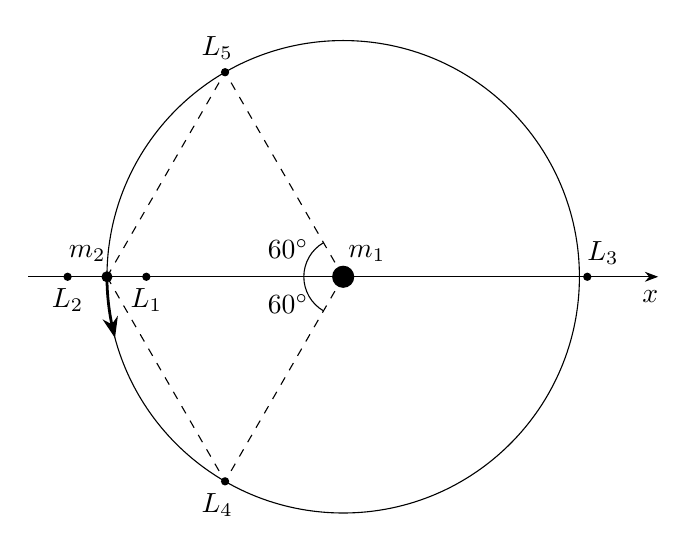
\begin{tikzpicture}[>=Stealth]
        \draw [->] (-4,0) -- (4,0);
        \draw (3.9,-0.25) node {$x$};
        \draw (0,0) circle [radius=3cm];
        \fill (0,0) circle [radius=4pt];
        \draw (0.3,0.3) node {$m_1$};
        \fill (-3,0) circle [radius=2pt];
        \draw [->,line width=1pt] (-3,0) arc [start angle=180,radius=3,delta angle=15];
        \draw (-3.25,0.3) node {$m_2$};
        \fill (-2.5,0) circle [radius=1.5pt];
        \draw (-2.5,-0.3) node {$L_1$};
        \fill (-3.5,0) circle [radius=1.5pt];
        \draw (-3.5,-0.3) node {$L_2$};
        \fill (3.1,0) circle [radius=1.5pt];
        \draw (3.3,0.3) node {$L_3$};
        \fill (-1.5,-2.5980762) circle [radius=1.5pt];
        \draw (-1.6,-2.9) node {$L_4$};
        \draw [dashed] (0,0) -- (-1.5,-2.5980762);
        \draw [dashed] (-3,0) -- (-1.5,-2.5980762);
        \fill (-1.5,2.5980762) circle [radius=1.5pt];
        \draw (-1.6,2.9) node {$L_5$};
        \draw [dashed] (0,0) -- (-1.5,2.5980762);
        \draw [dashed] (-3,0) -- (-1.5,2.5980762);
        \draw (-0.5,0) arc [start angle=180,radius=0.5,delta angle=60];
        \draw (-0.7,0.35) node {$60^\circ$};
        \draw (-0.5,0) arc [start angle=180,radius=0.5,delta angle=-60];
        \draw (-0.7,-0.35) node {$60^\circ$};
    \end{tikzpicture}
    \caption{\kaishu 二体系统中的五个Lagrange点的示意图（不按比例）}
\end{figure}

对于五个Lagrange点的有效势能可以进一步分析其极值的类型和Lagrange点附近的运动模式，详细的推导可以参见北京大学刘川教授的《理论力学》一书的第三章。经过计算我们发现\textbf{五个Lagrange点其实都对应有效势能的极大值}，但是由于Coriolis力的作用，$L_4$和$L_5$确实对于小的扰动是\textbf{稳定的}，而三个共线的Lagrange点附近的运动一般是\textbf{不稳定的}（非震荡解）。

事实上，要更为全面的理解在三个共线的Lagrange点附近的质点的运动，需要将其垂直于轨道平面的运动也考虑进来。在1968年的博士论文中，美国人Robert W. Farquhar首先考虑了地月系统$L_2$点附近的所谓晕轨道（halo orbit）。这是一个在$L_2$点附近的三维周期轨道。当时美国正在进行Appolo登月计划。Farquhar当时的研究是希望利用地月的$L_2$点来进行远程的通信，因为这个点可以同时连接地球和月球的背面。这可以作为后续在月球背面着陆的先期准备。不过这个计划后来并没有真正实施，美国也没有再推进诸如在月球背面登月的计划。最近，中国的嫦娥登月计划也利用了类似的设计在月球背面登月。与晕轨道类似的另一类三维的轨道称为Lissajous轨道。与晕轨道不同的是，这类轨道并不是严格周期的，而只是准周期的。该轨道在两个星体轨道平面内的投影按照所谓的Lissajous图形进行，因此得名。在共线的Lagrange点$L_2$附近，一般需要飞行器进行少许轨道位置调整（orbital station-keeping）。这类轨道已经多次运用在日地的Lagrange点$L_2$附近。最为著名的例如欧洲空间局（ESA）发射的Planck卫星。其主要任务是探测宇宙微波背景辐射（Cosmic Microwave Background，CMB）的各向异性。

总体来说，三个共线的Lagrange点并不是稳定的，但是在它们附近，卫星和探测器只需要较小的能量消耗就可以回复到平衡点。同时，由于这些Lagrange点距离地球比较近（相较于不共线的两个Lagrange点$L_4$和$L_5$而言），因此也被广泛地运用在空间探索之上。例如我国探月工程发射的鹊桥号中继卫星就运用了地月系统的Lagrange点$L_2$。

\chapter*{宇宙速度}

前面我们讨论了太阳系之中各个行星的基本情况，它们的轨道虽然一般来讲都是椭圆轨道，但是实际上绝大多数都十分接近于圆轨道。所以，在下面的讨论中假设所有行星的轨道都是围绕太阳运行的圆轨道是一个不错近似。另外，我们知道在每一个行星的Hill球内部的质点可以认为只受该行星的引力支配，而在每个行星的Hill球之外，质点则将只受太阳的引力支配。在太阳系，海王星有着最大的Hill球，半径是1亿1600万公里，或是$0.775\,\mathrm{AU}$；因为它与太阳距离的遥远，充分的补偿了它的质量低于木星的不足，木星的Hill球半径只有5300万公里。因此，以太阳系的尺度来看，我们基本上可以假定每个行星的Hill球基本上就是一个点，并且就位于该行星所在的位置。

这意味着，当我们讨论从某个行星（通常是指地球）发射人造星体在太阳系内旅行的时候，我们需要进行一次参照系的转换：首先，我们要以所在的行星为参照系，该人造星体必须脱离所在行星的引力束缚，逃逸到其Hill球之外；其次，我们应将参照系转换到太阳系（此时探测器的位置可以看作和行星位置一样），讨论该人造星体在太阳引力的影响下的进一步的运动。

我们首先来讨论人造星体环绕引力中心公转的最小速度问题。对于质量为$m$的一个人造星体，要使得它环绕一个半径为$R$、质量为$M$的球形行星的表面公转，它的最小速度为$v_R$，这称为该人造星体（在该行星上）的\textbf{环绕速度}。这可以由它所受的引力完全提供向心力获得，即：
\[
    \frac{mv_R^2}{R} = \frac{GMm}{R^2}
\]
得到：
\[
    \boxed{v_R = \sqrt{\frac{GM}{R}}}
\]
最为常用的例子是地球上的环绕速度。我们将$M$取为地球的质量$M_{\Earth}$，将$R$取为地球的半径$R_{\Earth}$，我们就得到地球表面的环绕速度，又称为\textbf{第一宇宙速度}：
\[
    v_{R,\Earth} = 7.91\,\mathrm{km/s}
\]
在地表发射的速度超过第一宇宙速度的人造星体，可以绕地球作Kepler轨道运动。

于是进一步讨论人造星体从一个引力中心逃逸的最小速度问题。对于质量为$m$的一个人造星体，要使得它从一个半径为$R$、质量为$M$的球形行星的表面逃逸，它的最小速度为$v_E$，这称为该人造星体（在该行星上）的\textbf{逃逸速度}。这可以由其总机械能为零获得，即：
\[
    \frac{1}{2}mv_E^2 - \frac{GMm}{R} = 0
\]
得到：
\[
    \boxed{v_E = \sqrt{\frac{2GM}{R}}}
\]
最为常用的例子是地球上的逃逸速度。我们将$M$取为地球的质量$M_{\Earth}$，将$R$取为地球的半径$R_{\Earth}$，我们就得到地球表面的逃逸速度，又称为\textbf{第二宇宙速度}：
\[
    v_{E,\Earth} = 11.19\,\mathrm{km/s}
\]
在地表发射的速度超过第二宇宙速度的人造星体，在摆脱了地球的引力之后可以到达地球Hill球外的太空（对地球的引力中心而言这等效于无穷远）。

假设我们不仅仅需要人造星体脱离地球的引力，我们还希望它能走得更远，比如说飞出太阳系。那么一般来说该星体需要更大的初始动能。具有第二宇宙速度的物体仅仅能够保证它克服地球的引力之后，飞到地球的Hill球之外。如果这个时候它相对于地球而言是静止的，它并不能够摆脱太阳的引力，而是会像地球一样围绕太阳运动。那么需要多少能量能够使其能够摆脱太阳的引力束缚呢？此时我们必须将参照系转换为太阳系。对一个处于地球公转轨道上质量为$m$的质点，它如果希望摆脱太阳的引力束缚，我们需要有：
\[
    \frac{1}{2}mv_{E,\Sun}^2 - \frac{GM_{\Sun}m}{a_{\Earth}} = 0
\]
其中$a_{\Earth}$是地球的公转轨道半径，这给出位于地球轨道半径处的一个质点从太阳系逃逸的速度$v_{E,\Sun}$：
\[
    v_{E,\Sun} = \sqrt{\frac{GM_{\Sun}}{a_{\Earth}}} = \sqrt{2}v_{\Earth}
\]
其中$v_{\Earth} = \sqrt{\dfrac{GM_{\Sun}}{a_{\Earth}}} = 29.78\,\mathrm{km/s}$是地球绕太阳公转的轨道速度。在我们下面的分析中会看到，将一个刚刚脱离地球引力的人造星体的速度用地球公转的轨道速度来度量是非常方便的。

因此，当我们从地球发射一个人造星体时，我们需要它在脱离了地球的引力之后仍然具有（相对于太阳而言）$\sqrt{2}v_{\Earth}$的速度，最经济的可能性显然是它相对于地球而言具有$(\sqrt{2}-1)v_{\Earth} = 12.34\,\mathrm{km/s}$的速度，这样在充分利用地球本身的公转速度$v_{\Earth}$之后恰好可以逃逸出太阳系。因此，如果我们以地球为参照系发射一个人造星体，要求它在摆脱了地球引力之后还能够摆脱太阳的引力并脱离太阳系，将其相对于地球的最小速度记为$u$的话，那么能量守恒告诉我们：
\[
    \frac{1}{2}mu^2 - \frac{GM_{\Earth}m}{R_{\Earth}} = \frac{1}{2}m(\sqrt{2}-1)^2 v_{\Earth}^2
\]
即：
\[
    \frac{1}{2}mu^2 - \frac{1}{2}mv_{E,\Earth}^2 = \frac{1}{2}m(\sqrt{2}-1)^2 v_{\Earth}^2
\]
这个式子与前面求解第二宇宙速度的公式的差别就在于，等式的右边不是零，而是一个正的动能。这保证了在摆脱了地球引力束缚之后，该人造星体还有剩余的动能。这个速度相对于地球而言恰好是$(\sqrt{2}-1)v_{\Earth}$。于是，在正确地叠加上地球本身的轨道速度$v_{E,\Earth}$之后，我们就可以获得逃逸太阳系所需要的逃逸速度$v_{E,\Sun} = \sqrt{2}v_{\Earth}$。因此我们最后得到，在地面上相对于地球而言最小的发射速度$u$满足：
\[
    \boxed{u = \sqrt{v_{E,\Earth}^2 + (\sqrt{2}-1)^2 v_{\Earth}^2}}
\]
这给出：
\[
    u = \sqrt{11.19^2 + 12.34^2} = 16.66\,\mathrm{km/s}
\]
它又被称为\textbf{第三宇宙速度}。

\chapter*{星际旅行}

本小节中我们将讨论太阳系内两个行星之间的旅行问题。如前所述，我们假定所有的行星都在圆轨道上围绕太阳公转。假设我们希望从轨道半径为$R_1$的行星表面发射一个人造星体，它在摆脱了所在行星的引力束缚之后，沿其Kepler轨道去造访轨道半径为$R_2$的另一个行星。我们该如何选择发射的速度以及时间?此外，这个星际旅行的时间需要持续多久等等这些问题都是必须考虑的。这方面典型的应用就是火星探测计划。当然，原则上我们也可以探测其他的行星。由于我们发射的行星一般总是在地球之上，因此我们一般总是取$R_1 = a_{\Earth} = 1\,\mathrm{AU}$。

一个几何上比较直观的事实是，由于任何人造星体的轨道都是以太阳为焦点的椭圆，因此最为简单的设定就是这个椭圆刚好以$R_1$和$R_2$为其近日点和远日点距离。换句话说，该椭圆刚好与两个行星的圆轨道相切于近日点和远日点。这被称为\textbf{Hohmann转移轨道}，一般也是最节省燃料的方案。根据椭圆的性质有$R_1 = a(1 - e)$，$R_2 = a(1 + e)$，因此我们可以得到该人造星体的半长轴$a$为：
\[
    a = \frac{1}{2}(R_1 + R_2)
\]
轨道偏心率为：
\[
    e = \frac{R_2 - R_1}{R_2 + R_1}
\]
以地球的火星探测计划为例，$R_1 = 1\,\mathrm{AU}$，$R_2 = 1.524\,\mathrm{AU}$，于是我们得到：$a = 1.262\,\mathrm{AU}$，$e = 0.2076$。有了这个数据已经可以直接获得旅行的时间了，诀窍就是利用Kepler第三定律。显然这个时间是椭圆轨道周期的\textbf{一半}，于是飞行器的旅行时间为：
\[
    t = \frac{1}{2}T_{\Earth}\cdot\left(\frac{a}{a_{\Earth}}\right)^{\tfrac{3}{2}} = \frac{1}{2} \times 1.262^{\tfrac{3}{2}} = 0.709\,\mathrm{a}
\]
也就是约260天或8.5个月。当然这只是个理想的估计，实际的火星探测过程中，人造的探测器是可以通过启动其发动机进行适当的轨道和速度调整的。但是这个数据仍然可以作为最节省能源的时长的一个不错的估计。发射途中只需两次引擎推进，探测器在地球轨道上瞬间加速后，进入椭圆形的Hohmann转移轨道。探测器由此椭圆轨道的近日点开始，抵达轨道远日点后再瞬间加速，进入火星的公转轨道并登陆火星。要注意的是，三个轨道的轨道半长轴是越来越大，因此两次引擎推进皆是加速，使探测器动能增加而进入能量较高（半长轴较大）的轨道。

我们前面看到，如果仅仅考虑与地球以及与太阳的两体相互作用，那么构造一个内切于地球和我们希望探测的星体圆轨道的Kepler椭圆轨道可以最节省能源地发射一个人造星体到太阳系内的任意一个行星。对于距离我们地球比较近的火星而言，这个Kepler轨道的飞行大约需要半年多的时间，仍然在可以接受的范围内。但是如果我们希望探索更加遥远的行星，比如说距离我们最远的海王星，那么这个方案就显得有些局促了。原因就在于，这个方法的飞行时间基本上完全由所在行星绕太阳的轨道半径所决定。对于太阳系中最外面的一颗行星，海王星的公转轨道半径为$a_{\Neptune} = 30.07\,\mathrm{AU}$。代入到上面的公式中，我们发现这个时间大约需要30.6年。尽管这还不是不可期待的长，但是对于一个航天计划而言，已经有些过于冗长了。最主要的原因是，航天计划一般是一个耗资巨大且涉及多方面科技的综合工程。在30年之中，很可能计划中所涉及的关键技术都会发生翻天覆地的变化，当初的设计早已过时。另一方面，国际和国内的政治、经济局势也可能发生剧烈的变化从而导致计划流产。因此，即使对于探测我们太阳系内部的行星而言，所需的时间还是应该尽可能地缩短一些为好。

好在理论上是存在一些办法的。一个奇特的解决方案就是所谓的\textbf{引力弹弓}方案。假设我们希望发射一个人造探测器去探测海王星，注意到在地球和海王星之间，存在这许多颇为巨大的行星，最典型的如木星、土星等。所谓引力弹弓方法就是设法让我们的探测器瞄准这些半路上的星体，使得它进入这些行星的引力场的范围。也就是说，我们力求探测器能够准确地进入木星的Hill球的范围之内。随后，我们需要选取木星为参照系。在这个参照系中，人造星体相对于木星而言，就是一个从无穷远入射的粒子在其引力势中的散射问题，基本结论是，对于力心（也就是木星）而言，入射的速率和出射的速率是完全相同的，但是方向会发射偏折。当人造星体摆脱了木星的引力范围后，它又重新回到太阳的引力范围内。这时候我们需要将参照系转换到太阳参考系之中。于是我们发现，在人造星体与木星接触并散射的前后，在太阳参考系来看，我们人造星体的速率大小实际上可能是增加的。尽管在木星的参考系来看，入射和出射速度是完全相同的。这部分多余的能量并不是凭空产生的，它实际上来源于木星的能量。只不过我们的人造星体太小，木星质量太大，因此它的能量损失可以忽略不计。但是对于我们的人造星体而言，从这个散射过程之中，它的确从木星那里“偷到”了一部分能量。剩下的运动过程中，人造星体继续以新的能量沿着Kepler轨道飞向海王星。由于获得了额外的动能，因此它比起不经过木星散射的轨道而言，可以更快地到达目的地。因此，总体而言，可以将整个飞往海王星的旅程分为三段：
\begin{itemize}
    \item[1.] 沿着Kepler轨道飞往木星轨道，确保其飞入木星的引力范围（Hill球）内
    \item[2.] 在木星的Hill球内，以木星为参照系与木星散射并再次飞出其引力范围
    \item[3.] 以新的速度沿着新的Kepler轨道继续飞往海王星
\end{itemize}
显然，要进行具体的计算并没有原则上的困难，只不过有些复杂而已。我们只需要分别利用前面的提及的方法，分为三段来进行具体的计算即可。当然，需要注意的是，在进行第二段的计算时，我们必须将参照系从太阳参照系转换到木星的参照系之中。在衔接第三段时又必须转换回去。仅就总的飞行时间而言，它除了依赖于飞行器刚刚脱离地球引力时的速度之外，很大程度上还依赖于我们能够多精确地使飞行器进入木星的Hill球以完成恰当的散射过程。散射过程所占的时长虽然可以忽略，但是恰当的散射可以使得探测器获得更多的额外动能，从而可以更快地到达海王星。如果我们能够比较精确的把瞄准距离调整到木星半径的几倍之内，详细的计算表明，最终的飞行时间将可以从原先的30年的时长缩减到10年以内。实际上，探测冥王星的“新视野”号探测器，只用了九年半时间就从地球到达了冥王星。

\end{document}
